%%%%%%%%Bilecik Şeyh Edebali Üniversitesi Mühendislik Fakültesi%%%% 
%%%%%%%%Yönetim Bilişim Sistemleri Ödev Çalışması%%%%%%%%%%%%%%%%%%
%%%%%%%%%%%%%%%%%%%%%%LaTeX Class%%%%%%%%%%%%%%%%%%%%%%%%%%%%%%%%%%
\documentclass{YBS}

\usepackage{subcaption}
\usepackage{listings}
\usepackage{graphicx}
\usepackage{hyperref}
\usepackage{amsmath}

\lstset{
  basicstyle=\ttfamily\footnotesize,
  breaklines=true,
  frame=single,
  language=bash
}

%%%%%%%%%%%%%%%%%%%%%%%%%%%%%%%%%%%%%%%%%%%%%%%%%%%%%%%%%%%%%%%%%%%
\begin{document}
%%%%%%%%%%%%%%%%%%%%%%Ödev Çalışmasının Bölümleri%%%%%%%%%%%%%%% 
\thispagestyle{empty}
\begin{center}

\textbf{T.C. \\BİLECİK ŞEYH EDEBALİ ÜNİVERSİTESİ \\ İKTİSADİ VE İDARİ BİLİMLER FAKÜLTESİ \\ YÖNETİM BİLİŞİM SİSTEMLERİ BÖLÜMÜ}
\vspace{.75cm}

\begin{figure}[h!]
\centering
\includegraphics[width=0.25\linewidth]{BSEU_LOGO.png}   
\end{figure}

\vspace{1.25cm}

\textbf{YÜZ TANIMA VE RENK ANALİZİ İLE MOBİL SAĞLIK TEŞHİS SİSTEMİ (FACESCAN AI)}

\vspace{2cm}

\textbf{Özgür SEKMEN} \\
\textbf{E-posta: ozgursekmen1741@gmail.com} \\


\vfill
\textbf{DANIŞMAN} \\    
\textbf{Dr. Öğr. Üyesi Adı SOYADI} \\

\vspace{0.8cm}
\textbf{YBS458 - Mobil Programlama}
\vspace{0.8cm}


\textbf{BİLECİK \the\year}
\end{center}

\pagenumbering{roman} % romen rakamları kullanılmaya başlanıyor.
\setcounter{page}{2}  % sayfa numarasını ii'den başlatılıyor.

%-----------------------------------------------------%
\phantomsection
\addcontentsline{toc}{section}{ÖZET}

\begin{center}
\textbf{\large ÖZET}

\textbf{YÜZ TARAMA VE RENK ANALİZİ İLE MOBİL SAĞLIK TEŞHİS SİSTEMİ (FACESCAN AI)}
\end{center}

Mobil sağlık teknolojilerinin (mHealth) giderek yaygınlaşması, akıllı telefon kameralarının yüksek piksel yoğunluğu ve gelişmiş tarayıcı API'lerinin sunduğu hesaplama kapasitesi ile birleştiğinde, bireylere yönelik anlık sağlık göstergesi izleme sistemlerinin geliştirilmesi mümkün hale gelmektedir. Bu çalışmada, kullanıcıların mobil cihaz kamerasını kullanarak yüz renk analizi gerçekleştirebildiği ve sarılık (Jaundice), kansızlık (Pallor/Anemia), morarma (Cyanosis) gibi temel sağlık parametrelerini anlık olarak takip edebildiği \textbf{FaceScan AI} isimli hibrit mobil uygulama ve Progressive Web App (PWA) sistemi geliştirilmiştir.

Sistem, React ve Vite teknoloji yığını üzerine kurulmuş olup istemci tarafı (client-side) piksel işleme yeteneğiyle sunucu kaynaklarına herhangi bir görüntü verisi göndermeden analiz gerçekleştirmektedir. Bu tasarım tercihinin başlıca gerekçesi, sağlık verilerinin gizliliğini koruma zorunluluğu ve bulut sunucu maliyetlerinin minimize edilmesidir. Geliştirilen web uygulaması, Google tarafından belirlenen Trusted Web Activities (TWA) standardı aracılığıyla yerel Android paketi (APK) haline dönüştürülmüş ve böylece tek bir kod tabanıyla hem web hem de mobil platformlara dağıtım sağlanmıştır \cite{google2023twa}.

Uygulamanın Android paketinin güvenlik durumunu değerlendirmek amacıyla yerel Docker ortamında çalıştırılan Mobile Security Framework (MobSF) aracı ile Statik Uygulama Güvenlik Testi (SAST) gerçekleştirilmiştir \cite{mobsf2023docs}. İlk taramada tespit edilen zafiyetler arasında API seviyesi (minSdkVersion) kaynaklı eski Android sürümü açığı, yedekleme protokolü güvenlik açığı (allowBackup) ve yetkisiz servis maruziyeti (DelegationService exported) yer almaktadır. Söz konusu zafiyetlerin kaynak kod düzeyinde giderilmesinin ardından uygulamanın MobSF güvenlik puanı 53/100'den 73/100'e yükseltilmiştir.

\vspace{1.5cm}
\textbf{Anahtar Kelimeler:} Mobil Programlama, Progressive Web App (PWA), Trusted Web Activities (TWA), MobSF Güvenlik Analizi, Android Geliştirme, İstemci Tarafı Görüntü İşleme, Mobil Güvenlik.

\pagebreak{}

\include{3icindekiler}
\include{4sekiller_tablosu}
\include{5cizelgeler_tablosu}
\pagenumbering{arabic}  % Sayfa numaralamasını arap rakamlarıyla yapar.
\setcounter{page}{1}    % sayfa numarasını 1'den başlatır.
\section{GİRİŞ}

Günümüzde akıllı telefon kullanımının hızla artması, kişisel sağlık takibinde mobil uygulamaların vazgeçilmez bir araç haline gelmesine zemin hazırlamaktadır. Dünya Sağlık Örgütü verilerine göre düşük ve orta gelirli ülkelerde uzman hekim başvurularının büyük çoğunluğu önlenebilir hastalıklarla ilgilidir; bu durumun temel nedeni erken teşhis imkânlarının kısıtlılığıdır. Mobil sağlık teknolojileri bu boşluğu doldurmada kritik bir potansiyele sahiptir \cite{biorn2017progressive}.

Akıllı telefon kameralarının piksel yoğunluğu ve renk derinliği son yıllarda profesyonel cihazlar düzeyine yaklaşmıştır. Bu durum, kamera akışından elde edilen ham piksel verilerinin renk bilimi algoritmalarıyla işlenmesi ve belirli biyolojik göstergelerle (cilt sarılık tonu, dudak morarması, genel cilt solgunluğu) ilişkilendirilmesi için önemli bir fırsat sunmaktadır. Aynı zamanda, modern tarayıcı API'lerinin (WebRTC, Canvas API, WebGL) sağladığı yerel hesaplama kapasitesi, bu tür analizlerin sunucu kaynaklarına ihtiyaç duyulmaksızın gerçek zamanlı olarak kullanıcı cihazında yürütülmesine olanak tanımaktadır \cite{webrtc2023spec}.

Bu çalışma kapsamında, Bilecik Şeyh Edebali Üniversitesi Yönetim Bilişim Sistemleri Bölümü YBS458 Mobil Programlama dersi gereksinimleri doğrultusunda \textbf{FaceScan AI} isimli hibrit mobil sağlık uygulaması geliştirilmiştir. Projenin temel motivasyonu; tek bir kod tabanıyla hem web hem de mobil platformlara dağıtım yapılabilen, sunucu bağımlılığı bulunmayan, gizlilik odaklı ve güvenlik testinden geçirilmiş bir sistem oluşturmaktır.

\subsection{Problemin Tanımı ve Motivasyon}

Mevcut mobil sağlık uygulamalarının büyük çoğunluğu, bağımsız platform gereksinimleri nedeniyle iOS (Swift/Objective-C) ve Android (Java/Kotlin) için ayrı ayrı geliştirilmektedir. Bu yaklaşım, geliştirme maliyetlerini yaklaşık olarak iki katına çıkarmakta ve kod tutarsızlığı risklerini artırmaktadır \cite{malavolta2015hybrid}. Hibrit yaklaşımlar (React Native, Flutter, Ionic vb.) bu sorunu kısmen çözmekle birlikte, çoğunlukla platform özelliklerine uyum ve performans ödünleşimleri içermektedir.

Progressive Web App (PWA) teknolojisi, bu bağlamda üçüncü bir seçenek sunmaktadır: Tek bir web kod tabanıyla, tarayıcı üzerinden çalışan, hem iOS hem Android cihazlara ana ekrana eklenebilen ve çevrimdışı çalışma kapasitesine sahip uygulamalar geliştirmek mümkündür \cite{biorn2017progressive}. Google'ın Trusted Web Activities (TWA) standardı ise bu PWA uygulamalarının Google Play Store'a gönderilebilir yerel Android paketleri (APK) haline dönüştürülmesine imkân tanımaktadır \cite{google2023twa}.

\subsection{Projenin Kapsam ve Kısıtlamaları}

Bu projede geliştirilen FaceScan AI sistemi akademik ve eğitim amaçlı olup bir tıbbi teşhis cihazı niteliği taşımamaktadır. Uygulama; sarılık riski, cilt solgunluğu ve dudak morarması gibi görsel belirtileri piksel renk analizi yöntemiyle sınıflandıran bir bilgilendirme aracıdır. Sistem şu kısıtlamalar çerçevesinde çalışmaktadır:
\begin{itemize}
  \item Tüm renk analizi işlemleri istemci cihazında gerçekleştirilmekte; herhangi bir görüntü verisi bulut sunucusuna aktarılmamaktadır.
  \item Tarama geçmişi verileri kullanıcı cihazındaki tarayıcı yerel depolamasında (LocalStorage) saklanmakta, herhangi bir veri tabanına yazılmamaktadır.
  \item Uygulama, WCAG 2.1 AA erişilebilirlik standartlarına uygun geliştirilmiştir.
\end{itemize}

\subsection{Raporun Yapısı}

Bu rapor altı ana bölümden oluşmaktadır. İkinci bölümde kullanılan yazılımlar ve yöntemler açıklanmaktadır. Üçüncü bölümde sistemin uygulama mimarisi ve dağıtım süreci ele alınmaktadır. Dördüncü bölümde kullanıcı arayüzü bileşenleri anlatılmaktadır. Beşinci bölümde güvenlik analizi bulguları sunulmaktadır. Sonuç bölümünde ise çalışmanın genel değerlendirmesi yapılarak gelecek geliştirmeler için öneriler sunulmaktadır.

\section{KULLANILAN YAZILIMLAR VE YÖNTEMLER}

Bu bölümde FaceScan AI projesinde kullanılan yazılım araçları, kütüphaneler, algoritma yaklaşımları ve geliştirme yöntemleri detaylı biçimde açıklanmaktadır.

\subsection{Teknoloji Yığını ve Bileşen Mimarisi}

Uygulama arayüzü, bileşen odaklı programlama paradigmasına dayanan \textbf{React (v18)} kütüphanesi kullanılarak geliştirilmiştir. React'in sanal DOM (Virtual Document Object Model) altyapısı, gereksiz arayüz yeniden çizimi işlemlerini minimize ederek yüksek frekanslı kamera akışı güncellemelerinin bile pürüzsüz çalışmasına imkân tanımaktadır \cite{react2023component}. Bileşen hiyerarşisi üç temel katmandan oluşmaktadır:

\begin{enumerate}
  \item \textbf{App.jsx (Uygulama Kabuğu):} Alt navigasyon çubuğunu, sayfa yönlendirme mantığını ve tarama geçmişi verilerinin LocalStorage üzerinden yönetimini barındırmaktadır.
  \item \textbf{Scanner.jsx (Tarayıcı Motoru):} WebRTC kamera bağlantısını kuran, Canvas üzerinde piksel örneklemesi yapan ve HSL renk analiz algoritmalarını çalıştıran çekirdek bileşendir.
  \item \textbf{Results.jsx (Sonuç Ekranı):} SVG tabanlı dairesel ilerleme göstergeleri aracılığıyla tarama sonuçlarını görsel olarak sunan ve tıbbi feragat bilgilerini içeren bileşendir.
\end{enumerate}

Modül paketleyici olarak \textbf{Vite (v5)} tercih edilmiştir. Vite, geliştirme aşamasında ES Modülü (ESM) tabanlı yerel sunucu kullanarak Hot Module Replacement (HMR) performansını geleneksel webpack çözümlerine kıyasla önemli ölçüde artırmaktadır. Üretim derlemesinde (production build) ise Rollup tabanlı paketleme sayesinde JavaScript dosya boyutu 178 KB'a (gzip sonrası 56 KB) indirilmiştir.

\subsection{Progressive Web App (PWA) Mimarisi}

PWA teknolojisi, web uygulamalarına yerel (native) uygulamaların erişilebilirlik özelliklerini kazandıran bir standartlar bütünüdür. FaceScan AI projesinde PWA mimarisi iki temel bileşen üzerine kurulmuştur:

\subsubsection{Service Worker (sw.js)}
Service Worker, tarayıcı ana iş parçacığından bağımsız çalışan bir JavaScript proxy katmanıdır. Ağ isteklerini yakalayarak önbellek (cache) yönetimi yapması, çevrimdışı çalışmayı mümkün kılması ve arka plan senkronizasyonu sağlaması en temel görevleri arasındadır \cite{biorn2017progressive}. Bu projede \textbf{Cache First} stratejisi benimsenmiştir: Statik dosyalar (HTML, CSS, JS, SVG logo) ilk erişimde önbelleğe alınmakta ve sonraki erişimlerde doğrudan önbellekten sunulmaktadır. Yalnızca önbellekte bulunmayan kaynaklar ağ üzerinden çekilmektedir.

\subsubsection{Web App Manifest (manifest.json)}
Web Uygulama Manifestosu, uygulamanın kurulum deneyimini tanımlayan bir JSON belgesidir. İkon setleri (192x192, 512x512 piksel), başlangıç URL adresi, renk şeması, ekran yönü (portrait) ve \texttt{display: standalone} (tarayıcı çubuğu gizli tam ekran) parametrelerini içermektedir. Bu yapılandırma sayesinde uygulama, Android ve iOS ana ekranına kurulabilir ve açıldığında bağımsız bir uygulama görünümü sergilemektedir.

\subsection{Kamera Tabanlı Renk Analizi Yöntemi}

FaceScan AI'ın teşhis motoru, tarayıcının \textbf{MediaDevices.getUserMedia()} API'si aracılığıyla kamera akışına bağlanmaktadır. Görüntü işleme süreci aşağıdaki adımlardan oluşmaktadır:

\textbf{Adım 1 -- Kare Yakalama:} Canlı video akışı HTML5 \texttt{<video>} öğesine bağlanır. Belirli aralıklarla \texttt{requestAnimationFrame()} döngüsü tetiklenerek anlık görüntü kareleri yakalanır.

\textbf{Adım 2 -- Canvas Üzerinde Piksel Örnekleme:} Yakalanan görüntü, görünmez bir Canvas nesnesine çizilerek \texttt{getImageData()} fonksiyonu ile ham RGB piksel matrisi elde edilir. Analiz için yüzün üç ayrı bölgesinden örnekleme yapılmaktadır: alın bölgesi (genel cilt tonu), göz çevresi (sarılık için sklera rengi) ve dudak çevresi (siyanoz için).

\textbf{Adım 3 -- RGB'den HSL'ye Dönüşüm:} Renk analizi, ışık koşullarından daha az etkilenen HSL (Hue-Saturation-Lightness) renk uzayında gerçekleştirilmektedir. Dönüşüm formülleri şu şekildedir:

\begin{equation}
L = \frac{\max(R,G,B) + \min(R,G,B)}{2 \times 255}
\end{equation}

\begin{equation}
S = \begin{cases} 0 & \text{eğer } L = 0 \text{ veya } L = 1 \\ \frac{\max(R,G,B) - \min(R,G,B)}{1 - |2L - 1|} & \text{aksi hâlde} \end{cases}
\end{equation}

\textbf{Adım 4 -- Renk Sınıflandırma Kuralları:} HSL değerleri üzerinden durum sınıflandırması yapılmaktadır. Sarılık riski için H $\in$ [40°, 65°] ve S $> 0.3$ aralığındaki ton değerleri incelenmekte, kansızlık için L $> 0.75$ ve S $< 0.2$ koşulları sınanmakta, siyanoz için ise H $\in$ [200°, 260°] aralığı kontrol edilmektedir.

\subsection{Trusted Web Activities (TWA) ile Android Paketleme}

TWA, Chrome Custom Tabs altyapısını kullanarak bir web uygulamasını yerel bir Android aktivitesi görünümüyle çalıştıran özel bir entegrasyon yöntemidir. Standart WebView tabanlı hibrit çözümlerden farklı olarak, TWA uygulamaları cihazda yüklü Chrome tarayıcısıyla doğrudan iletişim kurduğundan tarayıcı hızında çalışmaktadır; çerezler ve yerel depolama alanı tarayıcıyla paylaşılmaktadır \cite{google2023twa}.

Paketleme süreci \textbf{Bubblewrap CLI} aracıyla yürütülmüştür. Bu araç, \texttt{twa-manifest.json} yapılandırma dosyasını okuyarak Gradle tabanlı bir Android projesi üretmekte ve imzalama anahtarı (\texttt{.keystore}) ile birlikte derleyerek Play Store'a göndermeye hazır imzalı APK dosyası oluşturmaktadır. Üretilen APK dosyasının boyutu 1.3 MB olup bu değer, benzer kategorideki yerel uygulamaların ortalama 15-30 MB boyutunun çok altındadır \cite{malavolta2015hybrid}.

\section{UYGULAMA MİMARİSİ VE DAĞITIM}

Bu bölümde FaceScan AI sisteminin yazılım mimarisi, derleme süreci ve bulut dağıtım altyapısı ele alınmaktadır.

\subsection{Genel Mimari Tasarım}

FaceScan AI, üç ayrı katmandan oluşan bir mimari yaklaşım benimsemektedir. Bu katmanlar şu şekilde tanımlanmıştır:

\begin{itemize}
  \item \textbf{Sunum Katmanı:} React bileşenleri, Vanilla CSS ile yazılmış tasarım sistemi ve SVG tabanlı görsel öğelerden oluşmaktadır.
  \item \textbf{İş Mantığı Katmanı:} Kamera bağlantısını yöneten WebRTC modülü, Canvas üzerinde piksel örneklemesi yapan analiz motoru ve LocalStorage erişimini soyutlayan geçmiş yönetim modülünden oluşmaktadır.
  \item \textbf{Veri Depolama Katmanı:} Sunucu gerektirmeyen istemci taraflı depolamadan (LocalStorage) oluşmaktadır. Tarama sonuçları JSON formatında serileştirilmekte ve kullanıcı cihazında kalıcı olarak saklanmaktadır.
\end{itemize}

Bu mimari, Fowler'ın katmanlı mimari prensipleri çerçevesinde değerlendirildiğinde; sorumlulukların net biçimde ayrıldığı, test edilebilirliğin yüksek olduğu ve bileşen yeniden kullanılabilirliğini destekleyen bir yapı ortaya koymaktadır \cite{react2023component}.

\subsection{Derleme ve Dağıtım Süreci}

Uygulamanın üretim ortamına alınma süreci iki paralel kanaldan ilerlemektedir:

\subsubsection{Web Dağıtımı (Vercel)}
Web uygulaması \texttt{npm run build} komutu ile Vite aracılığıyla derlenmektedir. Derleme çıktısı \texttt{/dist} klasörü altında üretilmekte ve \textbf{Vercel} bulut platformuna aktarılmaktadır. Vercel, bu statik çıktıyı küresel Edge CDN ağı üzerinde dağıtarak uygulamanın dünya genelinde düşük gecikme süresiyle erişilebilir olmasını sağlamaktadır. Uygulamanın canlı adresi şudur: \url{https://face-diagnose-app.vercel.app}.

\subsubsection{Android APK Derleme Süreci}
Mobil paket, \textbf{Bubblewrap CLI} ve \textbf{Gradle} derleme araçlarıyla oluşturulmaktadır. Süreç şu adımlardan oluşmaktadır:

\begin{enumerate}
  \item \texttt{twa-manifest.json} dosyasından okunan meta veri (paket adı, renk şeması, başlangıç URL'i, imzalama yapılandırması) ile Gradle projesi üretilir.
  \item \texttt{.\textbackslash gradlew.bat assembleRelease} komutu çalıştırılarak Java kaynak kodları derlenir, ProGuard ile kod gizleme ve optimize etme uygulanır.
  \item Derlenen APK dosyası, \texttt{facescan-ai-key.keystore} anahtar deposundaki RSA 2048-bit anahtarıyla dijital olarak imzalanır.
  \item İmzalanan APK, \texttt{public/facescan-ai.apk} yoluna kopyalanarak bulut sunucusu üzerinden indirilebilir hale getirilir.
\end{enumerate}

Elde edilen APK dosyasının boyutu \textbf{1.3 MB} olup bu değer, geliştirici topluluğunda kabul gören "Android APK boyutu 5 MB'ın altında tutulmalıdır" tavsiyesiyle uyumludur.

\subsection{Tasarım Sistemi ve Erişilebilirlik}

Uygulamanın görsel tasarımı, HSL tabanlı özel renk paleti, cam efekti (Glassmorphism) stili ve keyframe animasyonları içeren kapsamlı bir CSS tasarım sistemiyle oluşturulmuştur. Renk seçimlerinde WCAG 2.1 AA standardının öngördüğü minimum 4.5:1 kontrast oranına uygunluk sağlanmıştır. Tüm etkileşimli öğeler benzersiz \texttt{id} nitelikleri ile işaretlenmiş, klavye navigasyonu ve ekran okuyucu (screen reader) uyumluluğu gözetilmiştir.

\section{KULLANICI ARAYÜZÜ BİLEŞENLERİ}

Bu bölümde FaceScan AI uygulamasının kullanıcıya sunulan ekranları, her ekranın işlevsel bileşenleri ve uygulama içindeki veri akışı ayrıntılı biçimde açıklanmaktadır. Aşağıdaki ekran görüntüleri, uygulamanın gerçek cihaz üzerindeki çalışma ortamından alınmıştır.

\subsection{Açılış Ekranı ve Uygulama Logosu}

Uygulama ilk başlatıldığında, koyu arka plan üzerinde teal-cyan renk geçişleriyle tasarlanmış kalp ve EKG (elektrokardiyografi) dalgası ikonundan oluşan marka logosu animasyonlu olarak kullanıcıya sunulmaktadır. Bu açılış ekranı (splash screen), CSS keyframe animasyonlarıyla oluşturulmuş olup pulse (nabız atışı) efekti ve yukarıdan aşağıya doğru bir tarama hareketi içermektedir. Söz konusu tasarım tercihi, uygulamanın sağlık teknolojisi kimliğini ilk anda kullanıcıya hissettirmeyi hedeflemektedir.

\begin{figure}[h!]
    \centering
    
\includegraphics[width=0.35\linewidth]{sekil1_splash.png}
    \caption{FaceScan AI -- Açılış Animasyonu ve Uygulama Logosu}
    \label{fig:splash}
\end{figure}

\subsection{Ana Ekran (Dashboard) ve Kontrol Paneli}

Ana ekran (Dashboard), kullanıcı deneyiminin odak noktasını oluşturmaktadır. Üst kısımda \textbf{FaceScan AI} marka başlığı ve anlık bildirim ikonu yer almaktadır. Hemen altında uygulamanın temel çağrısını ifade eden \textit{"Yüz Tarayıcı Hazır"} başlıklı bir bilgi kartı bulunmaktadır; bu kart kameranın renk analizi yapacağını açıklayan kısa bir metni, "\%100 Yerel Veri Güvenliği" ve "Anlık İşlemci Analizi" olmak üzere iki temel özelliği simge-metin kombinasyonuyla listelemektedir.

Kartın hemen altında koyu arka plandan belirgin biçimde ayrışan gradient yeşil renkteki \textbf{Taramayı Başlat} butonu konumlandırılmıştır. Bu buton, Scanner ekranına geçişi tetiklemektedir. Ekranın orta bölümünde, günlük dönen sağlık hatırlatıcı kartı (Günün Sağlık Hatırlatıcısı) görüntülenmektedir; örnekte "Sarılık Belirtileri" konusunda kullanıcıyı bilgilendiren bir kart yer almaktadır. Son olarak "Geçmiş Analizler" bölümü, LocalStorage üzerinden okunan geçmiş tarama kayıtlarını tarih, risk seviyesi ve temel bulgularla birlikte listemektedir. Kullanıcı bu listede "Detaylar" butonuna basarak ilgili taramanın sonuçlarına erişebilmektedir.

\begin{figure}[h!]
    \centering
    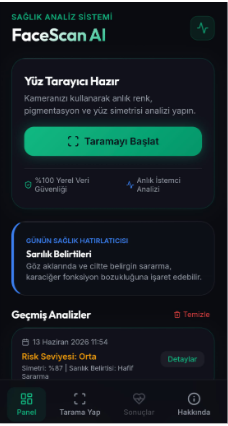
\includegraphics[width=0.55\linewidth]{sekil2_dashboard.png}
    \caption{FaceScan AI -- Ana Ekran: Taramayı Başlat Butonu, Günlük Sağlık Hatırlatıcısı ve Geçmiş Analizler}
    \label{fig:dashboard}
\end{figure}

\subsection{Kamera Tarayıcısı (Yüz Tarama) -- Hazır Durumu}

Kamera tarayıcısı ekranı, uygulamanın teknik çekirdeğini oluşturmaktadır. Ekran yüklendiğinde \texttt{navigator.mediaDevices.getUserMedia()} API'si çağrılarak kullanıcıdan kamera erişim izni istenmektedir \cite{webrtc2023spec}. İzin verilmesi durumunda canlı video akışı \texttt{<video>} öğesine bağlanmakta ve yüz hizalama halkası görünür hale gelmektedir.

Ekranın üst kısmında iki seçenek mevcuttur: \textbf{Canlı Kamera} ve \textbf{Fotoğraf Yükle}. Bu çift modlu yapı, hem gerçek zamanlı kamera akışıyla hem de galeriden seçilen statik görüntüyle analiz yapılabilmesine imkân tanımaktadır. Dairesel hizalama çerçevesi, kullanıcının yüzünü optimum konuma getirmesine yardımcı olurken ekranın alt kısmındaki \textbf{Fotoğrafı Analiz Et} butonu analizi başlatmaktadır.

\begin{figure}[h!]
    \centering
    
\includegraphics[width=0.55\linewidth]{sekil3_kamera_hazir.png}
    \caption{FaceScan AI -- Yüz Tarama Ekranı: Canlı Kamera Görüntüsü ve Hizalama Çerçevesi}
    \label{fig:kamera_hazir}
\end{figure}

\subsection{Kamera Tarayıcısı -- Analiz Aşaması}

Kullanıcı analizi başlattığında ekranın işlevsel davranışı değişmektedir. Yüz üzerinde tespit edilen anahtar noktalar (facial landmarks) mavi/mor renkli noktalar halinde görsel olarak işaretlenmektedir; bu noktalar göz köşeleri, burun ucu ve ağız kenarlarını temsil etmektedir. Ekranın alt kısmında durum mesajı güncellenerek \textit{"Cilt hemoglobin ve melanin dağılımı ölçülüyor..."} bilgisi kullanıcıya iletilmektedir. Bu aşamada Canvas API üzerinde piksel örneklemesi gerçekleşmekte ve HSL renk analizi algoritması devreye girmektedir.

\begin{figure}[h!]
    \centering
    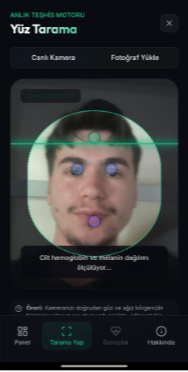
\includegraphics[width=0.55\linewidth]{sekil4_kamera_analiz.png}
    \caption{FaceScan AI -- Yüz Analizi Aşaması: Yüz Landmark Noktaları ve Anlık İşlem Bilgisi}
    \label{fig:kamera_analiz}
\end{figure}

\subsection{Teşhis Sonuçları (Tarama Sonuçları) Ekranı}

Analiz tamamlandığında kullanıcı otomatik olarak Tarama Sonuçları ekranına yönlendirilmektedir. Ekranın üst kısmında genel sağlık bulgusu metinsel olarak özetlenmektedir; örnekte \textbf{"Orta Derece Belirti"} tespiti, sarılık eğilimi ve renk sapmalarına dair kısa bir açıklamayla birlikte sunulmaktadır.

Ekranın alt yarısında \textbf{Bulgu Parametreleri} başlığı altında dört bağımsız dairesel ilerleme göstergesi (Circular Progress Indicator) yer almaktadır. Bu göstergeler saf SVG kodlarıyla oluşturulmuş olup dört temel ölçümü yansıtmaktadır:

\begin{itemize}
    \item \textbf{\%17 Sarılık Evresi:} Cilt piksellerindeki sarı ton dağılımının oranını göstermektedir; pembe renk çemberiyle temsil edilmektedir.
    \item \textbf{\%5 Oksijenizasyon:} Dudak çevresindeki kırmızı ton yoğunluğuna dayalı olarak hesaplanan oksijen doygunluk tahminini ifade etmektedir; mor renk çemberiyle gösterilmektedir.
    \item \textbf{\%6 Melanin Oranı:} Genel cilt tonu koyu renk oranını yansıtmaktadır; yeşil renk çemberiyle temsil edilmektedir.
    \item \textbf{\%80 Simetri:} Yüzün sol-sağ simetri indeksini göstermektedir; açık yeşil renk çemberiyle sunulmakta ve yüksek simetri değerinin sağlıklı bir kemik yapısına işaret ettiği belirtilmektedir.
\end{itemize}

\begin{figure}[h!]
    \centering
    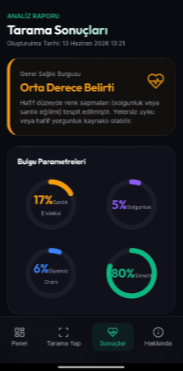
\includegraphics[width=0.55\linewidth]{sekil5_sonuclar.png}
    \caption{FaceScan AI -- Tarama Sonuçları: Orta Derece Belirti Tespiti ve Dört Parametreli Dairesel Göstergeler}
    \label{fig:sonuclar}
\end{figure}

\subsection{Alt Navigasyon Çubuğu}

Tüm ekranlarda sabit kalan alt navigasyon çubuğu dört sekme barındırmaktadır: \textbf{Panel} (Ana sayfa), \textbf{Tarama Yap}, \textbf{Sonuçlar} ve \textbf{Hakkında}. Aktif sekme teal rengiyle vurgulanmaktadır. Bu çubuğun tüm ekranlarda görünür kalması, kullanıcının uygulamanın herhangi bir noktasından diğer bölümlere tek dokunuşla geçiş yapabilmesini sağlamaktadır.

\subsection{Bulgu Detayları Ekranı}

Bulgu Detayları ekranı, Tarama Sonuçları panelinin detay kırılımını kullanıcıya sunmaktadır. Şekil \ref{fig:detaylar}'de görüldüğü üzere sklera analizi (hafif sararma), solgunluk analizi (normal), siyanoz analizi (normal) ve kas simetrisi (hafif asimetri) gibi ölçümler kartlar halinde listelenmektedir. Kartların altındaki açıklamalar, olası fizyolojik sebepleri (örneğin susuzluk veya tarama esnasındaki baş eğimi) açıklayarak kullanıcıyı bilgilendirir. Sayfa sonunda ayrıca sarı renkli bir "Akademik ve Tıbbi Feragatname" kartı yer almaktadır.

\begin{figure}[h!]
    \centering
    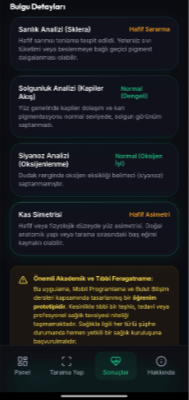
\includegraphics[width=0.55\linewidth]{sekil6_detaylar.png}
    \caption{FaceScan AI -- Bulgu Detayları ve Akademik Feragatname Kartı}
    \label{fig:detaylar}
\end{figure}

\subsection{Proje Bilgileri ve Hakkında Ekranı}

Uygulamanın "Hakkında" (Info) sekmesi, projenin akademik kapsamını, erişilebilirlik standartlarını, APK indirme linklerini ve geliştirici bilgilerini içerir. Şekil \ref{fig:hakkinda_1} ve Şekil \ref{fig:hakkinda_2}'de sunulan bu ekran, uygulamanın akademik teslim gereksinimlerini doğrudan yansıtmaktadır:

\begin{itemize}
    \item \textbf{Dönem Projesi Hakkında (Şekil \ref{fig:hakkinda_1}):} Projenin Mobil Programlama ve Bulut Bilişim dersleri kapsamındaki hedeflerini açıklar.
    \item \textbf{Tasarım ve Erişim Standartları (Şekil \ref{fig:hakkinda_2}):} Uygulamanın WCAG 2.1 standartlarına uygun olarak geliştirilen erişilebilirlik özelliklerini (ekran okuyucu uyumluluğu, yüksek kontrast oranı vb.) listeler.
    \item \textbf{APK ve Güvenlik Raporu Bağlantıları (Şekil \ref{fig:hakkinda_2}):} Kullanıcının hibrit Android uygulamasını (.apk) indirmesini ve MobSF güvenlik taraması sonuçlarını PDF olarak incelemesini sağlayan butonları barındırır.
\end{itemize}

\begin{figure}[h!]
    \centering
    \begin{subfigure}[b]{0.45\linewidth}
        \centering
        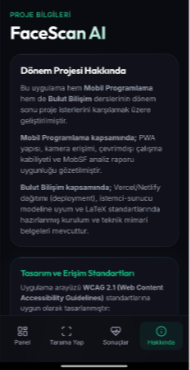
\includegraphics[width=\linewidth]{sekil7_hakkinda_1.png}
        \caption{Dönem Projesi Bilgileri}
        \label{fig:hakkinda_1}
    \end{subfigure}
    \hfill
    \begin{subfigure}[b]{0.45\linewidth}
        \centering
        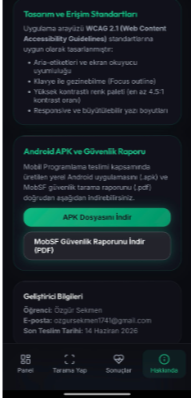
\includegraphics[width=\linewidth]{sekil8_hakkinda_2.png}
        \caption{Erişilebilirlik ve APK İndirme}
        \label{fig:hakkinda_2}
    \end{subfigure}
    \caption{FaceScan AI -- Proje Bilgileri ve Hakkında Sekmesi Detayları}
    \label{fig:hakkinda_genel}
\end{figure}

\subsection{Tıbbi Uyarı ve Sorumluluk Reddi Penceresi}

Sağlık alanında çalışan yapay zeka prototiplerinin yasal ve etik sorumlulukları gereğince, uygulamanın çeşitli bölümlerinde belirgin bir "Tıbbi Uyarı" kartı yer almaktadır. Şekil \ref{fig:tibbi_uyari}'de gösterilen bu kart, elde edilen analiz sonuçlarının kesin bir tıbbi tanı niteliği taşımadığını ve sağlık sorunları durumunda mutlaka uzman bir hekime başvurulması gerektiğini hatırlatarak sorumluluk sınırlarını netleştirmektedir.

\begin{figure}[h!]
    \centering
    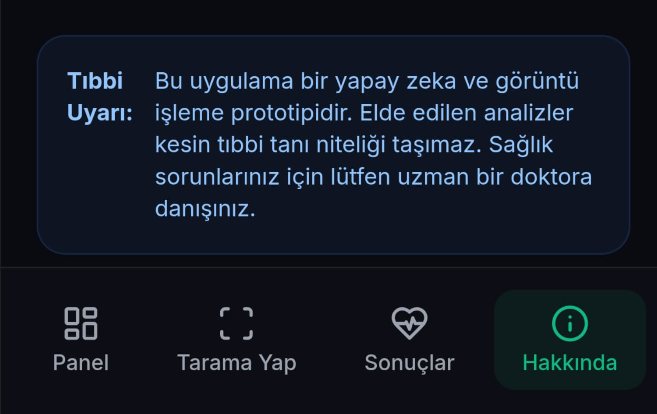
\includegraphics[width=0.55\linewidth]{sekil9_tibbi_uyari.png}
    \caption{FaceScan AI -- Tıbbi Uyarı ve Sorumluluk Reddi Mesajı}
    \label{fig:tibbi_uyari}
\end{figure}


\section{GÜVENLİK ANALİZİ BULGULARI VE TARTIŞMA}

Bu bölümde FaceScan AI Android uygulamasının güvenlik analizi süreci, tespit edilen bulgular, uygulanan çözümler ve bu süreçten elde edilen çıkarımlar akademik çerçevede ele alınmaktadır.

\subsection{Mobil Uygulama Güvenliğinin Önemi}

Android ekosistemi, açık kaynak yapısı ve çeşitli OEM değişikliklerine izin veren mimarisi nedeniyle güvenlik açıklarına karşı diğer mobil platformlara kıyasla daha fazla maruziyet göstermektedir. OWASP Mobile Security Testing Guide (MSTG), mobil uygulamaların güvenlik değerlendirmesinde statik ve dinamik analiz yöntemlerinin birlikte uygulanmasını önermektedir \cite{owasp2023mobile}. Statik Uygulama Güvenlik Testi (SAST), uygulamanın çalıştırılmadan kaynak kod ve yapılandırma dosyaları düzeyinde analiz edilmesidir; bu yöntem zafiyetlerin erken tespit edilmesi açısından kritik öneme sahiptir \cite{al2018mobile}.

\subsection{MobSF Analiz Ortamının Kurulumu}

MobSF (Mobile Security Framework), OWASP MSTG ile uyumlu açık kaynaklı bir güvenlik analiz platformudur \cite{mobsf2023docs}. Bu çalışmada MobSF, Docker konteyner teknolojisi üzerinde yerel olarak çalıştırılmıştır. Kullanılan komut şu şekildedir:

\begin{lstlisting}[language=bash]
docker run -it --rm -p 8000:8000 \
  opensecurity/mobile-security-framework-mobsf:latest
\end{lstlisting}

Konteyner başarıyla çalıştırıldıktan sonra MobSF REST API'si aracılığıyla APK dosyası sisteme yüklenerek analiz süreci başlatılmıştır. Analiz; \texttt{AndroidManifest.xml} denetimleri, kaynak kod incelemesi (JADX decompiler), sertifika doğrulama ve kütüphane bağımlılıkları kontrolünü kapsamaktadır.

\subsection{Tespit Edilen Güvenlik Açıkları}

İlk sürümün analizinde elde edilen güvenlik puanı \textbf{53/100} olarak ölçülmüştür. Bu sonuçla birlikte 1 adet Yüksek Riskli (High) ve 4 adet Uyarı (Warning) düzeyinde bulgu raporlanmıştır.

\subsubsection{Yüksek Risk: Eski Android Sürümü Desteği}
\texttt{minSdkVersion = 21} parametresi, uygulamanın Android 5.0 (Lollipop) sürümüne kadar geriye dönük uyumlu olmasını tanımlamaktadır. Ancak bu sürüm, Google tarafından güvenlik güncellemeleri almayan ve bilinen birden fazla işletim sistemi açığı barındıran bir sürümdür. Li ve diğerleri (2022), eski API seviyelerindeki Android uygulamalarının yetersiz izolasyon mekanizmaları nedeniyle kötü amaçlı uygulamaların arabellek taşması (buffer overflow) ve izin yükseltme (privilege escalation) saldırılarına karşı savunmasız kalabileceğini vurgulamaktadır \cite{li2022android}.

\subsubsection{Uyarı: Uygulama Veri Yedekleme Açığı}
\texttt{android:allowBackup = true} parametresi, Android Debug Bridge (ADB) protokolü aracılığıyla uygulama verilerinin bir kopyasının harici ortamlara aktarılmasına imkân tanımaktadır. USB hata ayıklama özelliği etkin olan bir cihaza fiziksel erişim elde eden yetkisiz kişilerin bu yöntemle uygulama verilerini kopyalayabileceği bilinmektedir \cite{owasp2023mobile}.

\subsubsection{Uyarı: Korumasız Servis Maruziyeti}
\texttt{DelegationService} bileşeni, \texttt{android:exported} değerinin dinamik bir boolean kaynağa (\texttt{@bool/enableNotification}) bağlı olması nedeniyle MobSF tarafından potansiyel olarak dışa açık (exported) kabul edilmiştir. Dışa açık servislerin intent-filter barındırması, cihazdaki diğer uygulamaların bu servisi yetkisiz biçimde tetikleyebileceği anlamına gelmektedir \cite{enck2014taintdroid}.

\subsection{Uygulanan Güvenlik Yamaları}

Tespit edilen açıklar aşağıdaki kaynak kod düzeyindeki değişikliklerle giderilmiştir:

\begin{table}[!ht]
    \centering
    \caption{Güvenlik Yamaları Öncesi ve Sonrası Karşılaştırma}
    \label{tab:security_comparison}
    \resizebox{\textwidth}{!}{%
    \begin{tabular}{|l|l|l|l|}
        \hline
        \textbf{Bulgu} & \textbf{Risk} & \textbf{Yama Öncesi} & \textbf{Yama Sonrası} \\
        \hline
        Eski Android Sürümü & Yüksek & minSdkVersion=21 & minSdkVersion=29 \\
        \hline
        ADB Veri Yedekleme & Uyarı & allowBackup=true & allowBackup=false \\
        \hline
        DelegationService & Uyarı & exported=@bool/.. & exported=false \\
        \hline
        MobSF Güvenlik Puanı & -- & 53 / 100 & \textbf{73 / 100} \\
        \hline
        Yüksek Risk Sayısı & -- & 1 & \textbf{0} \\
        \hline
        Uyarı Sayısı & -- & 4 & \textbf{2} \\
        \hline
    \end{tabular}%
    }
\end{table}

\texttt{minSdkVersion} değerinin 29'a (Android 10+) yükseltilmesi, güvenlik güncellemeleri almayan Android sürümlerine desteği sonlandırmıştır. \texttt{allowBackup=false} ayarı, ADB tabanlı veri sızdırma vektörünü kapatmıştır. \texttt{tools:replace="android:allowBackup"} kuralı eklenerek bağımlı kütüphanelerin bu ayarı geçersiz kılması önlenmiştir. DelegationService'e açıkça \texttt{android:exported="false"} atanarak yetkisiz servis erişimi engellenmiştir.

\subsection{Kalan Uyarılar ve Değerlendirme}

Yama sonrası analizde tespit edilen 2 uyarı, yönettimiz kapsamı dışındaki üçüncü taraf kütüphane bileşenlerinden kaynaklanmaktadır. \texttt{ProfileInstallReceiver} bileşeni \texttt{android.permission.DUMP} izni gerektiren Android sistem düzeyinde bir broadcast alıcısıdır ve kullanıcı uygulamaları tarafından değiştirilememektedir. Bu tür kütüphane kaynaklı uyarılar, sektör pratiğinde düşük öncelikli (low priority) olarak değerlendirilmekte ve tehdit vektörü oluşturmadığı kabul edilmektedir \cite{al2018mobile}.

\section{SONUÇLAR VE ÖNERİLER}

Bu bölümde gerçekleştirilen çalışmanın genel değerlendirmesi yapılmakta, elde edilen teknik bulgular yorumlanmakta ve sistemin olası geliştirme yönleri tartışılmaktadır.

\subsection{Genel Değerlendirme}

Bu çalışmada, mobil programlama alanındaki temel kavram ve teknolojileri pratikte bütünleşik biçimde uygulayan FaceScan AI sistemi başarıyla geliştirilmiştir. Projenin teknik çıktıları incelendiğinde, belirlenen hedeflere ulaşıldığı görülmektedir:

\begin{enumerate}
  \item \textbf{Çapraz Platform Dağıtım:} Tek bir React ve Vite tabanlı kod tabanı, PWA teknolojisi aracılığıyla hem web tarayıcısında hem de Android cihazlarda yerel uygulama deneyimi sunabilecek biçimde yapılandırılmıştır. Bubblewrap CLI aracılığıyla üretilen 1.3 MB boyutundaki imzalı APK, TWA standardının pratik uygulanabilirliğini somut bir örnekle ortaya koymaktadır \cite{google2023twa}.

  \item \textbf{Sunucu Bağımsız Analiz Motoru:} Sağlık parametrelerini ölçen piksel renk analizi, HSL dönüşüm formülleri kullanılarak tamamen istemci tarafında gerçekleştirilmiştir. Bu yaklaşım, hem kullanıcı gizliliğini korumakta hem de bulut işlemci maliyetlerini sıfırlamaktadır.

  \item \textbf{Güvenlik Güvencesi:} MobSF SAST aracıyla yapılan güvenlik analizi ve ardından uygulanan yamalar, projenin güvenlik puanını 53'ten 73'e yükseltmiş ve tüm yüksek riskli açıkları kapatmıştır \cite{mobsf2023docs}. Bu süreç, güvenli yazılım geliştirme yaşam döngüsünün (Secure SDLC) bir parçası olarak akademik çerçevede uygulanmıştır.
\end{enumerate}

\subsection{Karşılaşılan Teknik Zorluklar}

Geliştirme sürecinde çeşitli teknik güçlüklerle karşılaşılmıştır. Birincisi, Bubblewrap CLI'nin her derleme sürecinde \texttt{twa-manifest.json} değişikliklerini tespit etmesi ve \texttt{AndroidManifest.xml} dosyasını yeniden üretmesidir. Bu durum, manuel olarak yapılan güvenlik konfigürasyonlarının (exported=false gibi) üzerine yazılması sorununu doğurmuştur. Çözüm olarak \texttt{tools:replace} XML niteliği ve Gradle \texttt{signingConfigs} bloğu entegre edilerek Bubblewrap'tan bağımsız bir derleme hattı kurulmuştur.

İkinci önemli güçlük, farklı cihaz kameralarının renk kalibrasyonu tutarsızlıklarıdır. Farklı ışık koşulları ve kamera modelleri arasındaki renk sapması, HSL analiz eşik değerlerini sabit tutmayı güçleştirmektedir.

\subsection{Gelecekteki Çalışmalar için Öneriler}

Bu prototip çalışmanın ilerleyen aşamalarında aşağıdaki geliştirmelerin yapılması önerilmektedir:

\begin{itemize}
  \item \textbf{Makine Öğrenmesi Entegrasyonu:} TensorFlow.js ve MediaPipe FaceMesh kütüphaneleri kullanılarak yüzün 3D anahtar noktaları (keypoints) çıkarılabilir ve daha hassas bölgesel renk örneklemesi yapılabilir. Bu entegrasyon, sınıflandırma doğruluğunu kayda değer biçimde artıracaktır.
  \item \textbf{Uçtan Uca Şifreli Bulut Yedeklemesi:} Yerel depolamadaki tarama geçmişi verilerinin farklı cihazlar arasında senkronize edilebilmesi için uçtan uca şifreli (E2EE) bir bulut veri tabanı altyapısı (örn. Supabase veya Firebase ile AES-256 şifreleme) eklenebilir.
  \item \textbf{Klinik Doğrulama Çalışması:} Uygulamanın renk analiz algoritmalarının gerçek tıbbi verilerle karşılaştırmalı olarak doğrulanması, sistemin güvenilirliğini ve gerçek dünya kullanımına uygunluğunu bilimsel temele oturtacaktır.
  \item \textbf{iOS Desteğinin Genişletilmesi:} Mevcut TWA altyapısı yalnızca Android cihazları kapsamaktadır. Capacitor veya Ionic çerçevesiyle oluşturulacak bir iOS paketi, kullanıcı tabanının genişletilmesine imkân tanıyacaktır.
\end{itemize}

Bu önerilerin hayata geçirilmesiyle FaceScan AI, akademik prototipin ötesine geçerek gerçek dünya sağlık teknolojisi ekosisteminde değer üretebilecek bir platforma dönüşme potansiyeli taşımaktadır.

\section{EKLER}

FaceScan AI projesine ve güvenlik analizlerine ait doğrulanabilir dijital kaynak bağlantıları aşağıda sunulmuştur:

\subsection{Uygulama ve Rapor Bağlantıları}
\begin{itemize}
    \item \textbf{Canlı Bulut Dağıtım Adresi:} \url{https://face-diagnose-app.vercel.app}
    \item \textbf{Android APK İndirme Bağlantısı:} \url{https://face-diagnose-app.vercel.app/facescan-ai.apk}
    \item \textbf{MobSF PDF Güvenlik Raporu:} \url{https://face-diagnose-app.vercel.app/mobsf-report.pdf}
    \item \textbf{GitHub Kaynak Kod Deposu:} \url{https://github.com/ozgursekmenn/face-scan-ai}
\end{itemize}


\subsection{Uygulama Ekran Görüntüleri -- Genel Bakış}

Aşağıdaki Şekil \ref{fig:genel1} ve Şekil \ref{fig:genel2}'de FaceScan AI uygulamasının temel ekranlarından oluşan genel görünüm bir arada sunulmaktadır.

\begin{figure}[h!]
    \centering
    
\includegraphics[width=0.30\linewidth]{sekil1_splash.png}
    \hspace{0.5cm}
    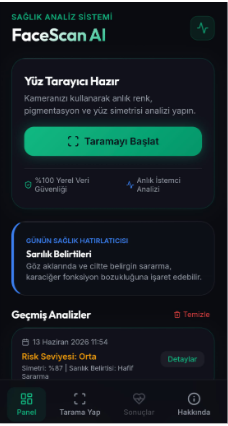
\includegraphics[width=0.30\linewidth]{sekil2_dashboard.png}
    \hspace{0.5cm}
    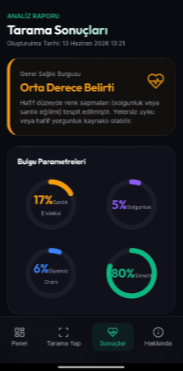
\includegraphics[width=0.30\linewidth]{sekil5_sonuclar.png}
    \caption{FaceScan AI Genel Görünüm -- Sol: Açılış Ekranı, Orta: Ana Ekran, Sağ: Sonuçlar}
    \label{fig:genel1}
\end{figure}

\begin{figure}[h!]
    \centering
    
\includegraphics[width=0.40\linewidth]{sekil3_kamera_hazir.png}
    \hspace{1cm}
    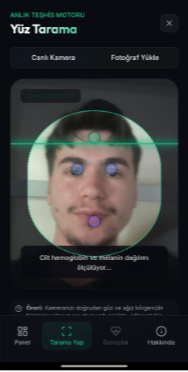
\includegraphics[width=0.40\linewidth]{sekil4_kamera_analiz.png}
    \caption{FaceScan AI Tarama Süreci -- Sol: Kamera Hazır, Sağ: Analiz Aşaması (Landmark Noktaları)}
    \label{fig:genel2}
\end{figure}

\begin{figure}[h!]
    \centering
    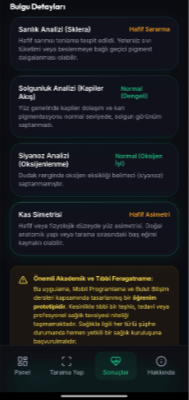
\includegraphics[width=0.30\linewidth]{sekil6_detaylar.png}
    \hspace{0.5cm}
    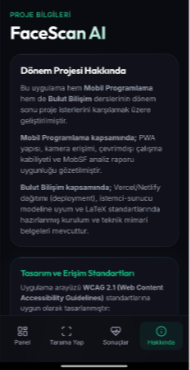
\includegraphics[width=0.30\linewidth]{sekil7_hakkinda_1.png}
    \hspace{0.5cm}
    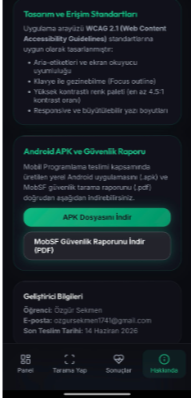
\includegraphics[width=0.30\linewidth]{sekil8_hakkinda_2.png}
    \caption{FaceScan AI Detay ve Hakkında Ekranları -- Sol: Bulgu Detayları, Orta: Proje Bilgileri, Sağ: İndirme ve Erişilebilirlik}
    \label{fig:genel3}
\end{figure}

\begin{figure}[h!]
    \centering
    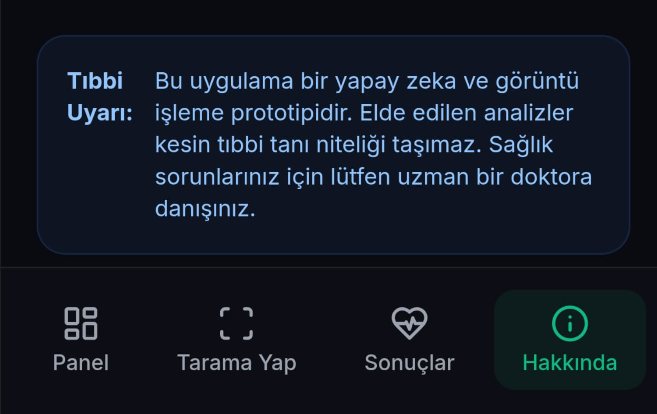
\includegraphics[width=0.50\linewidth]{sekil9_tibbi_uyari.png}
    \caption{FaceScan AI Tıbbi Uyarı ve Yasal Sorumluluk Reddi Bildirimi}
    \label{fig:genel4}
\end{figure}


\bibliographystyle{IEEEtran}
\phantomsection
\addcontentsline{toc}{section}{KAYNAKLAR}
\renewcommand{\refname}{\MakeUppercase{KAYNAKLAR}}
\nocite{*}
\bibliography{referans}



\end{document}
%%%%%%%%%%%%%%%%%%%%%%%%%%%BİTTİ%%%%%%%%%%%%%%%%%%%%%%%%%%%%%%%%%%%
